In diesm Kapitel werden alle wichtigen theoretischen Konzepte von Kanalkodierung und im speziellen zu Turbo-Kodes erklärt. Damit ist es möglich, die Implementation in C- beziehungsweise R-Code, welche in Kapitel~\ref{cha:implementation} erläutert wird, zu verstehen. Die Notation und der Inhalt orientieren sich an dem Buch von Schönfeld \cite{schoenfeld2012informations}.

Zuerst werden in Kapitel~\ref{sec:channelcoding} alle Grundlagen zur Kanalkodierung erläutert, welche dann bei der genauen Erklärung der Turbo-Kodes in Kapitel~\ref{sec:turboCodes} gebraucht werden.

\section{Kanalkodierung}
\label{sec:channelcoding}

\begin{figure}[th]
\centering
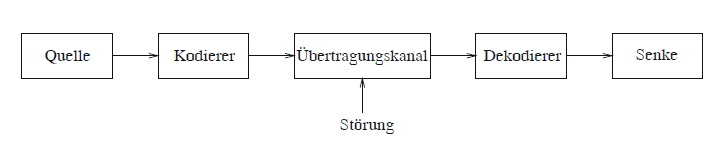
\includegraphics[width=\ScaleIfNeeded]{pictures/Channelmodel}
\caption{Modell der Nachrichtenübertragung,~Quelle:~\cite[10]{schoenfeld2012informations}}
\label{pic:channelmodel}
\end{figure}

In der Abbildung~\ref{pic:channelmodel} ist ein generelles Modell der Nachrichtenübertragung dargestellt, welches den Weg einer Nachricht zeigt. Nachdem der Sender (Quelle) die Nachricht durch den Quellenkodierer und Kanalkodierer geschickt hat, gelangt das Kanalwort auf den Übertragungskanal. Dort stören äußere Einflüsse das Signale und verändern es. Beim Empfänger (Senke) wird versucht, die Nachricht wieder zu dekodieren, um die Originalnachricht zu erhalten.

Das Ziel der Kanalkodierung dabei ist, den Quellenkodewörtern Redundanz hinzuzufügen, um nach einer fehlerhaften Übertragung über das Übertragungsmedium die Ausgangsnachricht wieder rekonstruieren zu können. Dabei können Fehler erkannt und im bestem Fall sogar komplett korrigiert werden.

Kanalkodierungen lassen sich in drei Kategorien unterteilen:

\begin{itemize}
\item Blockkodes
\item Faltungskodes
\item Turbo-Kodes
\end{itemize} 

Bei der ersten genannten Kategorie wird immer eine Nachricht einer bestimmten Länge kodiert. Bei Faltungskodes wird hingegen der ganzen Nachricht, unabhängig von der Länge, kontinuierlich Redundanz hinzugefügt. Turbo-Kodes andererseits verwenden bereits existierende Kodierer, wenden diese aber mehrfach an und vereinen das Ergebnis der Einzelnen.

\subsection{Zweites SHANNONsches Kodierungstheorem}
\label{sec:shannonTheorem}
Auf dem Übertragungskanal wird die zu übertragende Information zu einer bestimmen Wahrscheinlichkeit verfälscht. Durch die Kanalkodierung können Fehler bis zu einem bestimmten Grad korrigiert werden, jedoch bleiben Fehler mit einer bestimmten Restwahrscheinlichkeit.

SHANNON\footnote{Wurde nach Claude Elwood Shannon und Ralph Hartley benannt.} hat mit seinem zweitem Theorem bewiesen, dass es theoretisch möglich ist, eine Kanalkodierung zu finden, welche die Restfehlerwahrscheinlichkeit beliebig klein halten kann. Allerdings nur unter der Bedingung, dass der Sender weniger Kodewörter erzeugt, als der Kanaldekodierer beim Empfänger verarbeiten kann. Bereits 1948 erkannte SHANNON eine Grenze, die sogenannte SHANNON-Grenze, welche eine Grenze des Signal/Rausch-Verhältnisses, im Bezug auf die hinzugefügte Redundanz und der erreichbaren Restfehlerwahrscheinlichkeit darstellt. Somit wurde das Ziel gesteckt, mit einer geeigneten Kodierung, dieser Grenze möglichst nahe zu kommen. \cite[S.~125~f.]{schoenfeld2012informations}

Ein großer Schritt in Richtung dieser SHANNON-Grenze war die Vorstellung der Turbo-Kodes im Jahre 1993. Mit diesen war es erstmals möglich, dieser Grenze sehr nahe zu kommen. Vorgestellt wurde diese Art der Dekodierung in einem \emph{IEEE}-Artikel von Claude Berrou \cite{berrou1996near}.

\subsection{Prinzipien der Fehlerkorrektur}
\label{sec:principlesMistakesCorrection}
Das Anfügen von Redundanz kann auf ganz unterschiedliche Weisen erfolgen. Grundsätzlich gibt es 2 Möglichkeiten diese dem Quellenkodewort hinzuzufügen:

\begin{itemize}
\item Wiederholung der Nachricht
\item Rekonstruktion der Nachricht
\end{itemize}

Bei der ersten Möglichkeit fordert der Empfänger die Nachricht erneut an, wenn er bemerkt, dass die Nachricht nicht korrekt übertragen wurde. Er kann den Fehler durch Kontrollstellen in der Nachricht, zum Beispiel Paritätsbits, erkennen. Bei der zweiten Möglichkeit dient die hinzugefügte Redundanz nicht nur der Erkennung der Fehler, sondern auch als Hilfe zur Rekonstruktion der Originalnachricht. Natürlich hier muss die Redundanz größer sein, als bei der ersten Methode, die nur Fehler erkennt.

Es wird vorausgesetzt, dass die Wahrscheinlichkeit von Einzelfehlern größer ist, als das Auftreten von Bündelfehlern, also mehrere Fehler hintereinander. Jede Kodierung hat seine Grenzen, deswegen kann auch der beste Dekodierer nicht unendlich viele Fehler korrigieren. Zur Rekonstruktion des Kodewortes wird die \emph{Maximum-Likelihood-Methode} verwendet. Dabei wird das Kodewort gesucht, das einem existierenden, realistischen Wort am nähesten liegt. Dadurch liefert der Dekodierer immer ein Kodewort, welches die geringste Distanz zum gesendeten Kodewort aufweist. Das bedeutet jedoch nicht, dass dies unbedingt die richtige Nachricht sein muss. Jedoch steigt der Berechnungsaufwand dieser Methode mit der Länger der Nachricht enorm an.~\cite[126-129]{schoenfeld2012informations} 

\subsection{Verwendete Notation}
\label{sec:notation}
In den folgenden Kapiteln werden immer wieder Variablen verwendet, welche hier eingeführt und anschließend immer benützt werden, ohne sie bei der konkreten Formel nochmals anzuführen. Bei diesen Definition werden immer Kodewörter mit dem Alphabet $\{0,1\}$ verwendet, da dieser Fall am meisten Bedeutung hat.

Nachrichten werden zuerst mit dem Quellenkodierer in eine möglichst redundanzfreie Form gebracht, um die verwendeten Bits möglichst gut auszunutzen. Diese Kodewörter werden als Quellenkodewörter bezeichnet und sind folgenderweise definiert:

\begin{t_def}
Ein Wort $a^* \in \{0,1\}^l$ wird als Quellenkodewort der Länge $l$ bezeichnet.
\end{t_def}

Im Anschluss wird durch den Kanalkodierer Redundanz den Quellenkodewörtern hinzugefügt. Das resultierende Kodewort sieht folgendermaßen aus:

\begin{t_def}
Ein Wort $a \in \{0,1\}^n$ wird als Kanalkodewort der Länge $n$ bezeichnet.
\end{t_def} 

Durch das Hinzufügen von Redundanz ergeben sich $k = n - l$ redundante Stellen. Diese werden zur Fehlererkennung und Fehlerkorrektur bei der Dekodierung verwendet.

\begin{e_exa}
Gegeben sei eine Nachricht vom Quellenkodierer der Länge $l=2$, $a^*_{1}=(00),a^*_{2}=(01),a^*_{3}=(10),a^*_{4}=(11)$. Danach fügt der Kanalkodierer eine redundante Stelle $k=1$ hinzu. Somit haben die Nachrichten dann eine Länge von $n=3$. Sie könnten folgenderweise aussehen, $a_{1}=(001),a_{2}=(010),a_{3}=(100),a_{4}=(110)$.
\end{e_exa}

\subsection{Kenngrößen von Kanalkodes}
\label{sec:channelParameters}
Für die Betrachtung von verschiedenen Kanalkodierungen ist es wichtig, Unterscheidungsmerkmale zu finden. Dazu wird als erstes in Kapitel~\ref{sec:hammingDistance} die Distanz zwischen zwei Kodewörtern erklärt, um im Anschluss in Kapitel~\ref{sec:hammingWeight} das Gewicht eines Wortes berechnen zu können. Zuletzt wird in Kapitel~\ref{sec:codeRate} wird noch der Begriff der Koderate eingeführt.

\subsubsection{Hamming-Distanz}
\label{sec:hammingDistance}
Damit durch einzelne Fehler auf dem Übertragungskanal nicht eine andere existierende Nachricht produziert wird, sollen Kodewörter angestrebt werden, die sich möglichst weit voneinander unterscheiden. Eine wichtige Kenngröße dabei ist der Abstand zwischen zwei Kodewörtern.

\begin{t_def}
Die Anzahl der Stellen, in denen sich 2 Kodewörter $a_i$ und $a_j$ unterscheiden, bezeichnet man als \emph{Hamming-Distanz} zwischen den beiden Wörtern.
\end{t_def} 
 
\begin{equation}
d(a_i,a_j) = \sum^{n}_{g=1} (a_{ig} \oplus a_{jg})
\label{eq:hammingDistance}
\end{equation}

Diese lässt sich bei Binärkodes mit der Formel~\ref{eq:hammingDistance} berechnen. Dabei wird einfach gezählt, wie viele Stellen sich unterscheiden. Interessant ist der kleinste Unterschied zwischen zwei Kodewörtern, diese Zahl wird \emph{minimale Hamming-Distanz} $d_{min}$ genannt.

Ein Kode der alle Verfälschungen $\leq f_e$ erkennen kann, muss eine \emph{minimale Hamming-Distanz} von 

\begin{equation}
d_{min} = f_e + 1
\end{equation}

besitzen. Mit $f_e$ lässt sich der Grad der Fehlererkennung beschreiben. Die Anzahl der korrigierbaren Fehler $f_k$ lässt sich folgendermaßen berechnen:

\begin{equation}
f_k = \frac{d_{min}-1}{2}
\end{equation}

Damit nun Fehler erkannt und korrigiert werden können, muss die \emph{minimale Hamming-Distanz} mindestens folgende Gleichung erfüllen:~\cite[S.~132~f.]{schoenfeld2012informations}

\begin{equation}
d_{min} = f_e + f_k + 1
\end{equation} 

\subsubsection{Hamming-Gewicht}
\label{sec:hammingWeight}
Ein weiterer Zusammenhang zwischen der \emph{Hamming-Distanz} und den zu korrigierende Fehler, beschreibt das \emph{Hamming-Gewicht}.

\begin{t_def}
Anzahl der 1er in einem binären Kodewort $a=(a_1,a_2,\dotsc)$.
\begin{equation}
w(a) = \sum^n_{j=1} a_j
\label{eq:hammingWeight}
\end{equation} 
\end{t_def} 

Zur Berechnung dieses Gewichtes kann die Formel~\ref{eq:hammingWeight} verwendet werden. Solange 

\begin{equation}
d(a_i,b)=w(a_i \oplus b) = w(e) \leq f_k
\end{equation} 

kann das Kanalkodewort korrigiert werden. Dabei entspricht $b$ einem existierenden Kanalkodewort und $a_i$ der zu korrigierenden Nachricht.~\cite[134]{schoenfeld2012informations}
\subsubsection{Koderate}
\label{sec:codeRate}
Um ein Maß zu bekommen, wieviel Redundanz der Nachricht bei einem Kodierer hinzugefügt wird, wurde die Koderate eingeführt.

\begin{t_def}
Das Verhältnis der Längen zwischen Quellenkodewort $a^*=(a^*_1,a^*_2,\dotsc,a^*_l)$ und Kanalkodewort $a=(a_1,a_2,\dotsc,a_n)$ wird Koderate genannt.
\begin{equation}
R = \frac{l}{n} \leq 1
\end{equation} 
\end{t_def} 

Eine hohe Koderate zeigt, dass wenig Redundanz hinzugefügt wurde und somit weniger Fehler korrigiert werden können. Dagegen hat eine niedrige Koderate den Vorteil, dass sehr viele Fehler bei der Übertragung wiederherstellbar sind.~\cite[136]{schoenfeld2012informations} 

\subsection{Modell eines Übertragungskanal}
\label{sec:channels}
Um Nachrichten an den gewünschten Empfänger zu transportieren, können verschiedene Übertragungsmedien, wie zum Beispiel Kupferkabel oder Funkwellen, verwendet werden. Jedes dieser hat spezielle Eigenschaften und Charakteristiken. Damit diese Übertragungsmedien mit einem Computerprogramm simuliert werden können, muss ein Modell geschaffen werden, welches einen solchen Übertragungskanal bestmöglich abbildet. Dieses Modell bildet alle Störungen und Dämpfungen ab, die während der Übertragung auftreten können. Als ein gut geeignetes Modell stellte sich das Überlagern des Signals mit dem \emph{Additiv Weißes Gaußsches Rauschen} (AWGR) heraus \cite[81]{schoenfeld2012informations}. Dieses Rauschen wird wie folgt berechnet:

\begin{equation}
E_s = \frac{1}{L} \displaystyle\sum_{i=0}^{L-1} |x[i]|^2; \quad L = length(x)
\label{eq:power}
\end{equation}

In der Formel~\ref{eq:power} wird zuerst die Länge der Nachricht berechnet, um im Anschluss über alle Bits zu iterieren und die Summe der Quadrate des Signals zu berechnen. Diese Summe wird anschließend noch durch die Länge dividiert, um die Leistung je Bit zu erhalten.

\begin{equation}
noise = \sqrt{\frac{E_s}{10^{dB/10}}} * randn(1,L)
\label{eq:noise}
\end{equation}

Das Signal/Rausch-Verhältnis muss zuerst vom Dezibel-Bereich in den Linearen umgerechnet werden, wie im Nenner der Wurzel in der Gleichung~\ref{eq:noise} zu sehen ist.
Zur Berechnung des Rauschens werden $L$ Zufallszahlen zwischen 0 und 1 erzeugt und diese mit dem Wurzelergebnis multipliziert. 

\begin{equation}
y = x + noise
\label{eq:noisySignal}
\end{equation}

Danach wird einfach das Rauschen mit dem Originalsignal überlagert, um das verrauschte Signal zu erhalten. Dieses stellt nun den simulierten Übertragungskanal dar. Die Stärke der Störung kann mittels der $dB$-Variable beeinflusst werden.~\cite{AWGN}

\section{Turbo-Kodes}
\label{sec:turboCodes}
Mit der Einführung von Mobilfunk und Satellitenkommunikation wurden neue Kodes benötigt, die auch zufällig verteilte Einzelfehler und lange Bündelfehler korrigieren können. Eine Lösung dieses Problems sah man in der Verkettung mehrerer bereits existierender Kodes. Dabei werden die Vorteile der einzelnen Kodes genutzt, um einen noch leistungsfähigeren Gesamtkode zu erhalten, der mit Einbeziehung der Soft-Werte (also den realen Signalpegel beim Eingang des Dekodierers) einen Durchbruch in Richtung der SHANNON-Grenze darstellt. Bei der Dekodierung wird die Nachricht iterativ, also mehrmals durch die selben Dekodierer geschickt, um so eine Verbesserung der Ergebnisse zu erzielen.~\cite[S.~242~f.]{schoenfeld2012informations}

Die ersten Versuche wurden mit der seriellen Verkettung versucht, welche auch heute noch in der Anwendung sind. Beim klassischen Turbo-Kode werden jedoch parallel verkettete Faltungskodes verwendet, die iterativ dekodiert werden. Diese Art der Turbo-Kodes wurden auch in dieser Bachelorarbeit verwendet. Deshalb wird in Kapitel Kapitel~\ref{sec:parallelConvCodes} auch nur diese Art genauer erklärt.

\subsection{Parallel verkettete Faltungskodes} 
\label{sec:parallelConvCodes}
Bei der parallelen Verkettung von Faltungskodes werden meistens systematische (ein Ausgang wird durchgeschalten) rekursive Faltungskodierer verwendet, die nur wenige Register besitzen.

\begin{figure}[th]
\centering
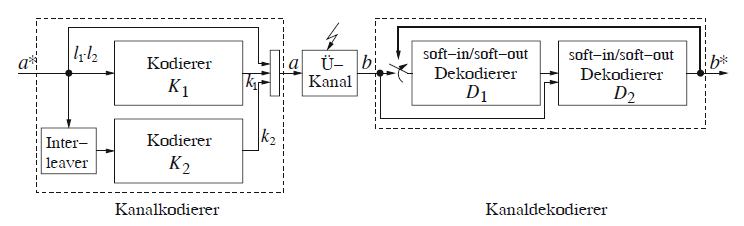
\includegraphics[width=\ScaleIfNeeded]{pictures/TurboModel}
\caption{Schema der parallelen Kodeverkettung,~Quelle:~\cite[251]{schoenfeld2012informations}}
\label{pic:turbomodel}
\end{figure}

Bei der Kodierung wird, wie in Abbildung~\ref{pic:turbomodel} zu sehen, das Quellenkodewort $a^*$ in den Kodierer $K_1$ und permutiert in den Kodierer $K_2$ geschickt. Das resultierende Kanalkodewort $a$, wird dann aus dem originalen Quellenkodewort $a^*$ und den beiden kodierten Nachrichten $k1$ und $k2$ gebildet. Bei der Wahl der Interleaver gibt es verschiedene Ansätze, wie die Bits permutiert werden, damit eine größtmögliche Distanz $d_{min}$ zwischen den Kodewörtern erreicht wird. Der einfachste Interleaver ist jener, der die Bits zufällig austauscht, wobei Sender und Empfänger den Permutationsvektor kennen müssen. Die verschiedenen Arten werden in Kapitel~\ref{cha:implementation} genauer erklärt. Am Ende der Kodierung kann noch Punktierung angewendet werden, um die Koderate zu erhöhen. Dieses Verfahren wird in Kapitel~\ref{sec:puncturing} genauer erläutert.

\begin{e_exa}
Angenommen das Quellenkodewort ist $a^*=(100)$ und die beiden kodierten Nachrichten sind $k1=(110)$ und $k2=(001)$, dann setzt sich das resultierende Kanalkodewort folgenderweise zusammen $a=(110010001)$. Dabei werden zuerst alle ersten Bits ausgegeben, dann die Zweiten und am Ende die Dritten.
\end{e_exa}

Da bei der Übertragung die Nachrichten als Spannungen interpretiert werden, ist es vonnöten die Nachrichten auf die Signalpegel -1 und +1 zu transformieren. Dabei wird die folgende Abbildungsvorschrift verwendet:

\begin{equation*}
	\begin{cases}
	-1 & \quad \text{wenn Bit}=1\\
	1 & \quad \text{wenn Bit}=0\\
	\end{cases}
\end{equation*}

Die Rückwandlung in 0er und 1er erfolgt erst nach der Dekodierung, da der Soft-In/Soft-Out Dekodierer die genauen Signalpegel bei Berechnung der Zuverlässigkeitswerte verwendet. 

\begin{figure}[th]
\centering
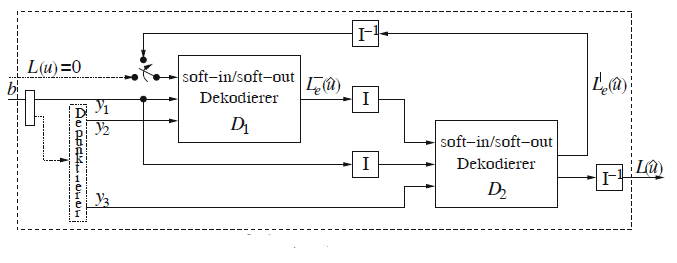
\includegraphics[width=\ScaleIfNeeded]{pictures/TurboDecoderSchema}
\caption{Aufbau der Dekodierschaltung,~Quelle:~\cite[262]{schoenfeld2012informations}}
\label{pic:decoderSchema}
\end{figure}

Auf der Abbildung~\ref{pic:decoderSchema} ist der Dekodierer detaillierter zu erkennen. Dabei erkennt man, dass am Anfang die Depunktierung und das Aufspalten der Nachricht in die drei Bestandteile erfolgt. Die gesamten Interleaver $I$ und Deinterleaver $I^{-1}$ werden benötigt, um die korrekte Reihenfolge der Bits herzustellen. Auf diesem Schema ist sehr gut zu erkennen, dass die extrinsischen Informationen aus den Dekodierern $L^-_e(\widehat{u})$ und $L^|_e(\widehat{u})$ in den Eingang des Nächsten geschickt werden. Bei der ersten Iteration wird noch 0 in den ersten Dekodierer geschickt, bei weiteren Iterationen wird die Rückkopplung verwendet.

Zur Berechnung der extrinsischen Informationen kann entweder der MAP-Algorithmus \cite[233-236]{schoenfeld2012informations} oder der aufwandsgünstigere Soft-Output VITERBI-Algorithmus \cite[222-233]{schoenfeld2012informations} verwendet werden. Die genaue Berechnung der extrinsischen Informationen kann im Buch von Schönefeld \cite[S.~263~f.]{schoenfeld2012informations} nachgeschlagen werden. Auch die Bachelorarbeit von Martin Nocker~\cite[7-11]{nocker} liefert Aufschluss über die Berechnung der Soft-Output-Werte beim VITERBI-Algorithmus.

Am Ende der Iterationen kann die Zuverlässigkeitsinformation berechnet werden:

\begin{equation}
L(\widehat{u}(i))=y_1(i)+L^-_e(\widehat{u}(i))+L^|_e(\widehat{u}(i))
\label{eq:resultDecode}
\end{equation}

Mit dem in der Formel~\ref{eq:resultDecode} berechneten Zuverlässigkeitswert, können die geschätzten Informationsbits abgeleitet werden:

\begin{equation*}
\begin{cases}
0 & \quad L(\widehat{u}(i)) \geq 0 \\
1 & \quad \text{sonst}
\end{cases}
\end{equation*}

Daraus wurde nun die Originalnachricht rekonstruiert und steht dem Empfänger zur Verfügung. Versuche zeigen, dass Turbo-Kodes mit kleiner Registeranzahl ($\leq 5$), sehr langen Eingangsfolgen ($2^{16}$) und mit 10-20 Iterationen, eine Leistungsfähigkeit nahe der SHANNON-Grenze erreichen.~\cite[265]{schoenfeld2012informations}

Turbo-Kodes sind aus der heutigen Zeit nicht mehr wegzudenken, da sie in fast allen Bereichen eingesetzt werden. Nur mehr bei Anwendungen, bei denen die Dekodierungsverzögerung sehr klein sein muss, werden noch klassische Kodes eingesetzt.

\begin{figure}[th]
\centering
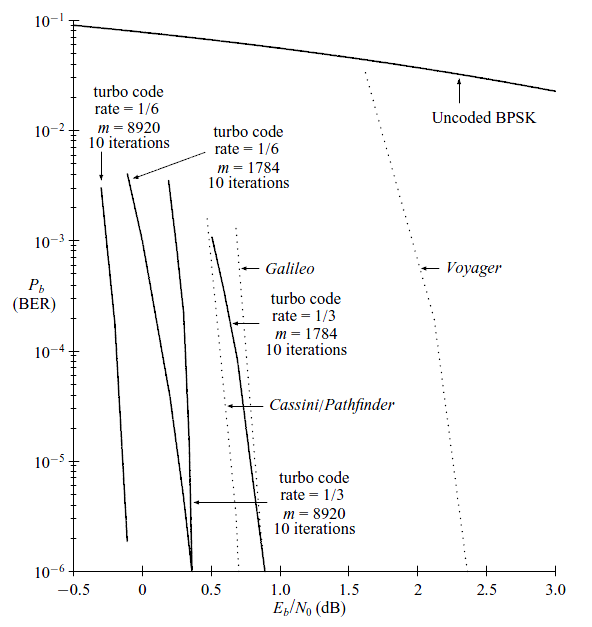
\includegraphics[width=\ScaleIfNeeded]{pictures/ComparisonTurbo}
\caption{Vergleich von verschiedenen Turbo-Kodes,~Quelle:~\cite[603]{huffman2010fundamentals}}
\label{pic:comparisonTurbo}
\end{figure}

Die Abbildung~\ref{pic:comparisonTurbo} zeigt eine Grafik, bei der auf der Ordinate die Bitfehlerrate und auf der Abszisse das Signal/Rausch-Verhältnis  aufgetragen sind. Aufgetragen sind verschiedene Turbo-Kodes mit verschiedenen Parametern. Es ist zu erkennen, dass eine längere Nachricht zu einer Verbesserung des Ergebnisses führt. Bei steigender Iterationsanzahl sinkt die Bitfehlerrate, jedoch steigt die Verzögerungszeit für das Dekodieren. Je mehr Iterationen durchgeführt werden, desto näher kommt man der SHANNON-Grenze.

\FloatBarrier
\subsection{Punktierung}
\label{sec:puncturing}
Wenn der Übertragungskanal besser als erwartet ist und noch Leistungsreserven vorhanden sind, kann Punktierung eingesetzt werden. Dabei werden Bits vor der Übertragung nach einer genauen Vorschrift (Punktierungsmatrix) gelöscht und vor der Dekodierung wieder eingefügt. Diese $m \times \frac{p}{m}$ Punktierungsmatrix $P$  wird spaltenweise durchlaufen und an den 0 Stellen werden die Bits gelöscht und ansonsten bleiben sie erhalten. Die Matrix muss bei Turbo-Kodes immer drei Zeilen haben, um bei der Dekodierung wieder ein eindeutiges Ergebnis zu liefern. Die resultierende Koderate erhält man folgenderweise:

\begin{equation}
R_p = \frac{p}{w(P)} * \frac{1}{3}
\end{equation} 

Die generelle Koderate bei Turbo-Kodes ist gleich $\frac{1}{3}$, da die Nachrichtenlänge verdreifacht wird. Darum findet sich diese Zahl auch in der Berechnung der Koderate mit Punktierung wieder.~\cite[218]{schoenfeld2012informations}

\begin{e_exa}
Angenommen die Kanalkodefolge ist $a=(101101011)$ und zur Erhöhung der Koderate wird folgende Punktierungsmatrix $$P_{3 \times \frac{6}{3}}=\begin{pmatrix}
1 & 0 \\
0 & 1 \\
1 & 1
\end{pmatrix}$$ angewendet. Die punktierte Kanalkodefolge ist dann $a_p=(1*1*010*1)=(110101)$. Die Koderate wird auf $R_p = \frac{6}{4} * \frac{1}{3} = \frac{1}{2}$ erhöht. 
\end{e_exa}